\documentclass[t]{beamer}
%\documentclass[t,handout]{beamer}
\usepackage[utf8]{inputenc}  % to be able to type unicode text directly
%\usepackage[french]{babel}   % french typographical conventions
\usepackage{inconsolata}     % for a nicer (e.g. non-courier) tt family font
%\usepackage{amsthm,amsmath}  % fancier mathematics
\usepackage{array} % to fine-tune tabular spacing
\usepackage{bbm} % for blackboard 1

\usepackage{graphicx}        % to include images
%\usepackage{animate}         % to include animated images
\usepackage{soul}            % for colored strikethrough
%\usepackage{bbding}          % for Checkmark and XSolidBrush
\usepackage{hyperref,url}

\colorlet{darkgreen}{black!50!green}  % used for page numbers
\colorlet{darkgray}{black!50!gray}
\definecolor{term}{rgb}{.9,.9,.9}     % used for code insets

\setlength{\parindent}{0em}
\setlength{\parskip}{1em}


% coco's macros
\def\R{\mathbf{R}}
\def\F{\mathcal{F}}
\def\x{\mathbf{x}}
\def\y{\mathbf{y}}
\def\u{\mathbf{u}}
\def\Z{\mathbf{Z}}
\def\d{\mathrm{d}}
\DeclareMathOperator*{\argmin}{arg\,min}
\DeclareMathOperator*{\argmax}{arg\,max}
\newcommand{\reference}[1] {{\scriptsize \color{gray}  #1 }}
\newcommand{\referencep}[1] {{\tiny \color{gray}  #1 }}
\newcommand{\unit}[1] {{\tiny \color{gray}  #1 }}

% disable spacing around verbatim
\usepackage{etoolbox}
\makeatletter\preto{\@verbatim}{\topsep=0pt \partopsep=0pt }\makeatother

% disable headings, set slide numbers in green
\mode<all>\setbeamertemplate{navigation symbols}{}
\defbeamertemplate*{footline}{pagecount}{\leavevmode\hfill\color{darkgreen}
   \insertframenumber{} / \inserttotalframenumber\hspace*{2ex}\vskip0pt}

%% select red color for strikethrough
\makeatletter
\newcommand\SoulColor{%
  \let\set@color\beamerorig@set@color
  \let\reset@color\beamerorig@reset@color}
\makeatother
\newcommand<>{\St}[1]{\only#2{\SoulColor\st{#1}}}
\setstcolor{red}

% make everything monospace
\renewcommand*\familydefault{\ttdefault}

\begin{document}

\begin{frame}[plain,fragile]
\Large\begin{verbatim}




     Fonctions de Mathieu :
     Modélisation, Analyse et Simulation






enric.meinhardt@ens-paris-saclay.fr
rafael.grompone@ens-paris-saclay.fr
\end{verbatim}
\end{frame}

\addtocounter{framenumber}{-1}
\begin{frame}
Dualité onde/corpuscule~:

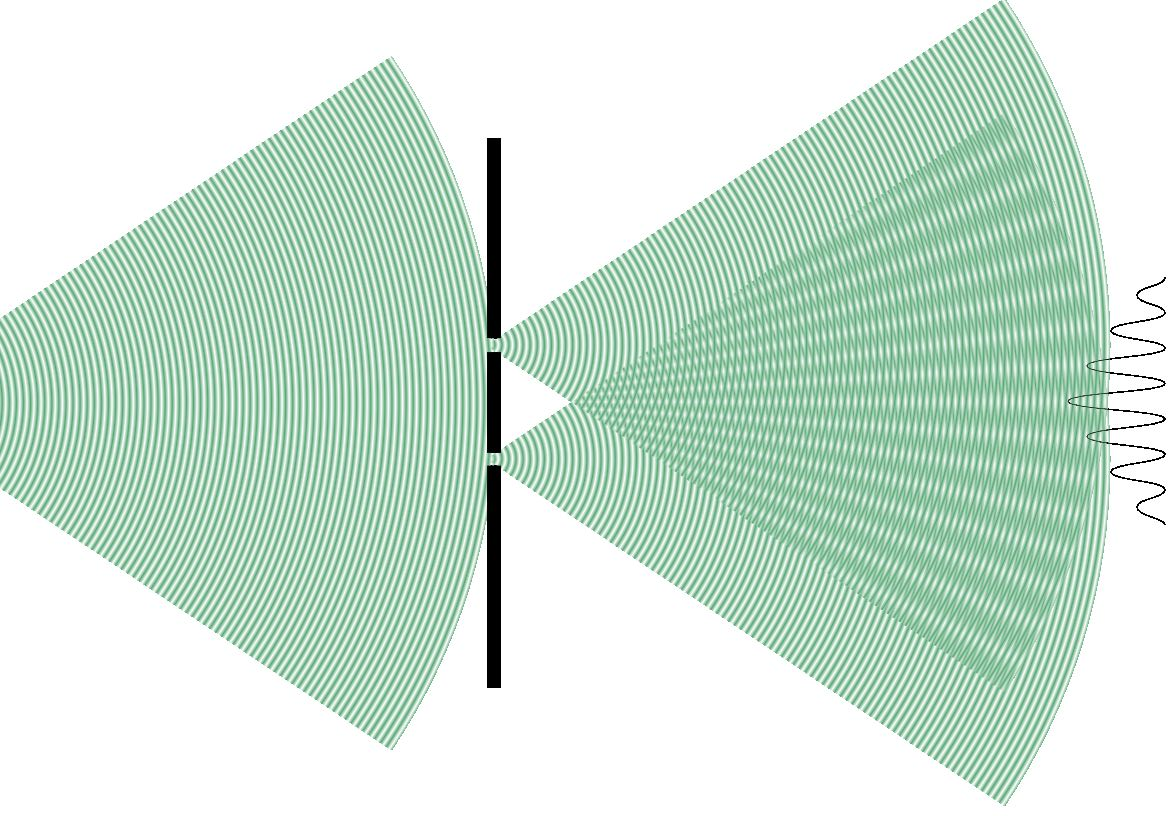
\includegraphics[height=0.36\textheight]{f/fentes.jpg}\hfill%
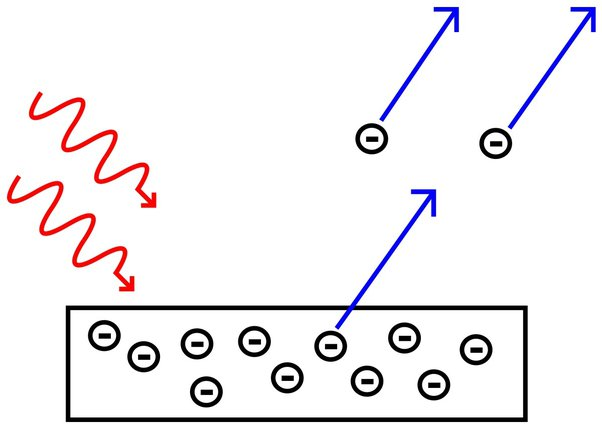
\includegraphics[height=0.36\textheight]{f/photoelectric.jpeg}


\vfill
\pause
Dualité billard/tambour~:

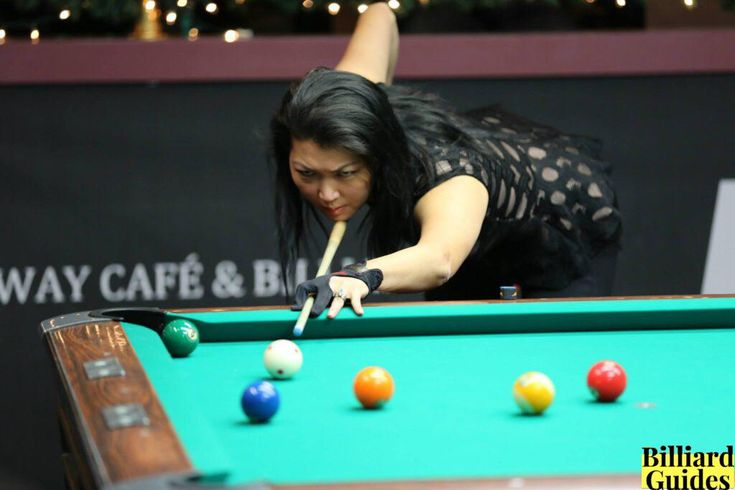
\includegraphics[height=0.38\textheight]{f/jeanette.jpg}\hfill%
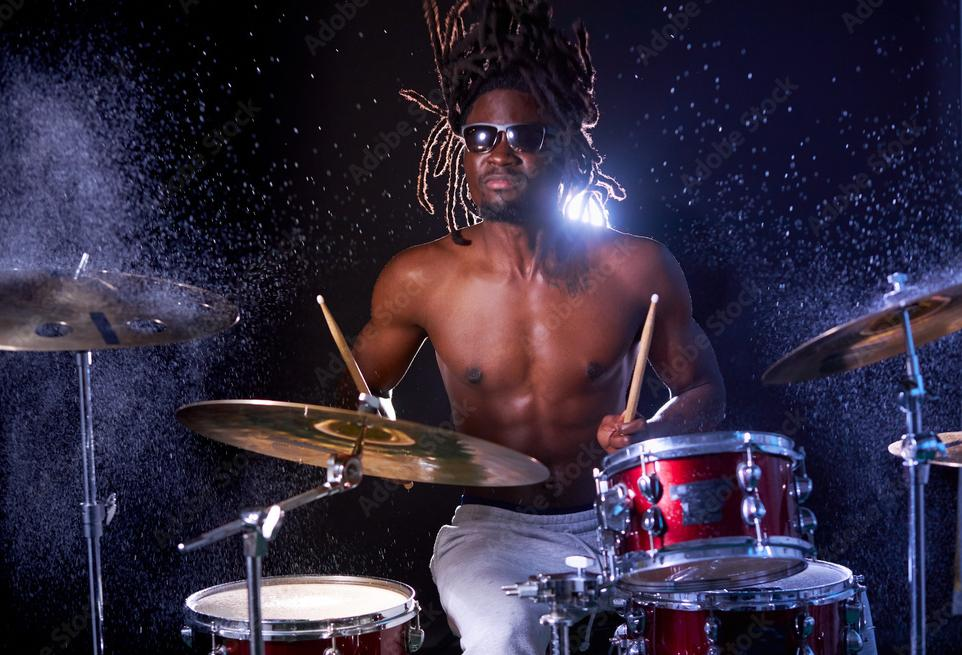
\includegraphics[height=0.38\textheight]{f/drummer.jpg}
\end{frame}

\begin{frame}
CAS D'UN DOMAINE ELLIPTIQUE\\
===========================

Types de trajectoires dans un billard elliptique~:

\begin{tabular}{cccc}
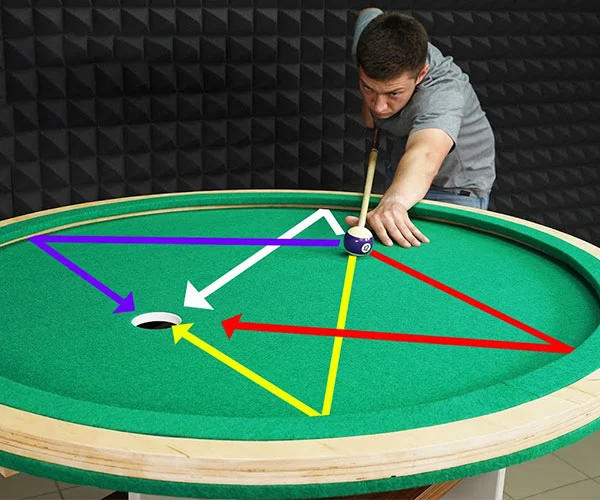
\includegraphics[width=0.23\textwidth]{f/billard_elliptique.jpg}&
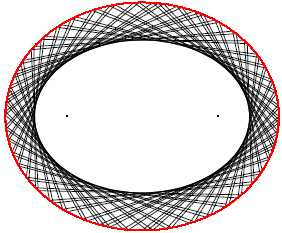
\includegraphics[width=0.23\textwidth]{f/traj1.png}&
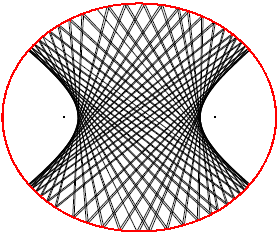
\includegraphics[width=0.23\textwidth]{f/traj2.png}&
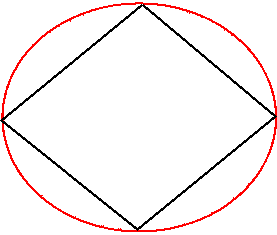
\includegraphics[width=0.23\textwidth]{f/trajp.png}\\
\scriptsize\color{darkgray} foyer-foyer &
\scriptsize\color{darkgray} rasante &
\scriptsize\color{darkgray} centrale &
\scriptsize\color{darkgray} périodique
\end{tabular}

\vfill

\pause

Types de modes de vibration d'un tambour elliptique~:
\begin{tabular}{cccc}
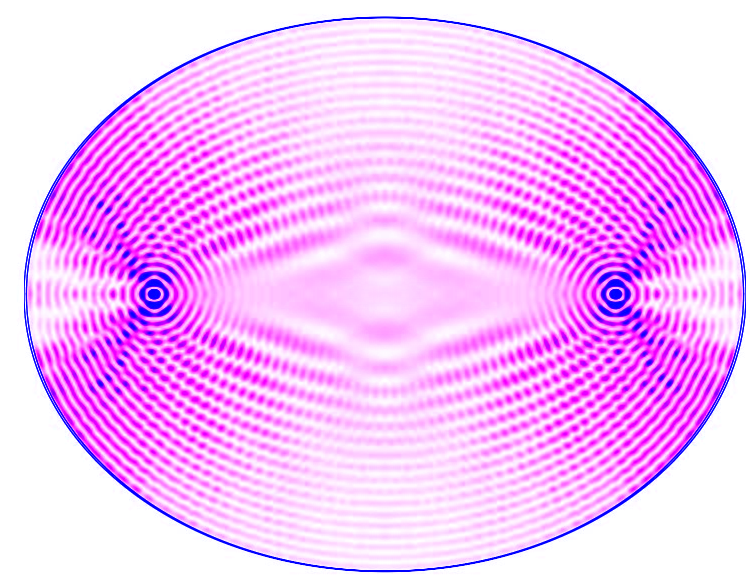
\includegraphics[width=0.23\textwidth]{f/foci2.png}&
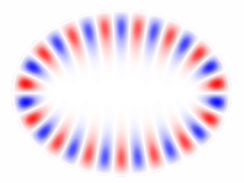
\includegraphics[width=0.23\textwidth]{f/whisper3.png}&
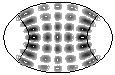
\includegraphics[width=0.23\textwidth]{f/bouncing.png}&
\only<3>{
\includegraphics[width=0.13\textwidth]{f/questionmarkp.png}}\\
\scriptsize\color{darkgray} foyers &
\scriptsize\color{darkgray} "whispering" &
\scriptsize\color{darkgray} localisé &
\scriptsize\color{darkgray} périodique
\end{tabular}

\end{frame}

\begin{frame}
ÉQUATIONS\\
=========

Équation de Helmholtz~:% dans un domaine elliptique~$\Omega$~:
\(
	\begin{cases}
		\Delta {\color{red}\bf u} = -{\color{red}\bf \lambda u} & \qquad\Omega \\
		{\color{red}\bf u} = 0 & \qquad\partial\Omega
	\end{cases}
\)

Coordonnées elliptiques~:
\(
	\begin{cases}
		x = {\color{darkgreen}c} \cosh\rho\cos\theta \\
		y = {\color{darkgreen}c} \sinh\rho\sin\theta \\
	\end{cases}
\)~\raisebox{-1em}{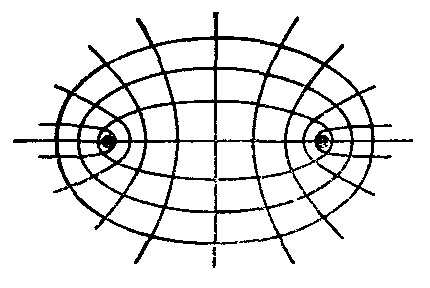
\includegraphics[width=0.14\linewidth]{f/elicords.png}}

Équations de Mathieu~:
\(
	\begin{cases}
		{\color{blue}f}''+({\color{darkgreen}a_i}-2{\color{darkgreen}q_i}\cosh(2\rho)){\color{blue}f} = 0\\
		{\color{blue}g}''-({\color{darkgreen}a_k}-2{\color{darkgreen}q_k}\cosh(2\theta)){\color{blue}g} = 0
	\end{cases}
\)

%\small
Solutions~:~$\begin{cases}{\color{red}\bf u}_{i,j,k,l}(\rho,\theta)={\color{blue}f_i}({\color{darkgreen}\alpha_{j}}\rho){\color{blue}g_k}({\color{darkgreen}\beta_{l}}\theta)\\ {\color{red}\lambda}_{i,j,k,l}=({\color{darkgreen}\alpha_{j}}^2+{\color{darkgreen}\beta_{l}}^2)/{\!\!\cdot\!\!\cdot\!\!\cdot}\end{cases}$

\vfill
\scriptsize
${\color{blue}f_i}$: fonctions de Mathieu radiales\\
${\color{blue}g_i}$: fonctions de Mathieu angulaires\\
${\color{darkgreen}\alpha_j,\beta_l}$: racines de Mathieu
%\pause
\color{darkgreen}$\Longleftarrow\ $\bf premier objectif du stage

\end{frame}



\begin{frame}
FONCTIONS DE MATHIEU ET MODES ELLIPTIQUES\\
=========================================

{
\scriptsize
\begin{tabular}{cc}
	Mathieu radiale~${\color{blue}f_5}(\rho)$ &
	Mathieu périodique~${\color{blue}g_{46}}(\theta)$\\
	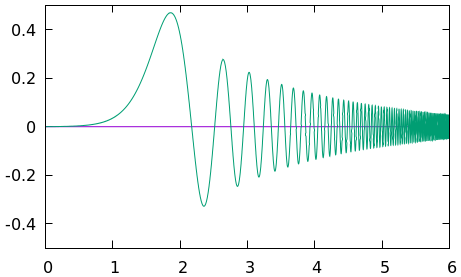
\includegraphics[width=0.43\linewidth]{f/mathieu_radial.png} &
	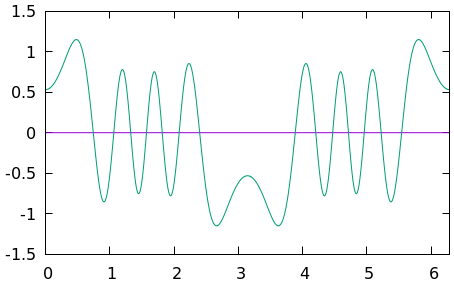
\includegraphics[width=0.43\linewidth]{f/mathieu_periodic.png} \\
\end{tabular}
}

\begin{columns}[c]
	\begin{column}{0.5\linewidth}
%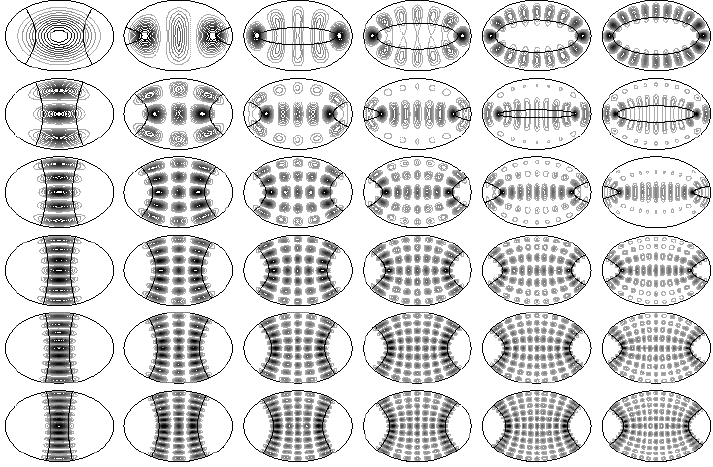
\includegraphics[width=0.53\linewidth]{f/contourplotsf.png}\\
		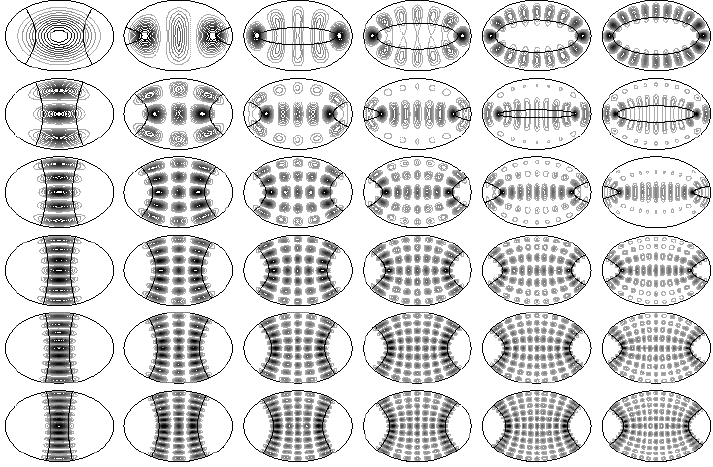
\includegraphics[width=\linewidth]{f/contourplotsf.png}\\
		\tiny\color{darkgray}
		Waalkens-Wiersig-Dullin, {\bf Elliptic Quantum Billiard},
		Annals of Physics 2016
	\end{column}
	\begin{column}{0.5\linewidth}
		\tiny\color{darkgray}
		Aucun des logiciels mathématiques librement disponibles
		(GNU Scientific Library, SciPy, Octave, etc.) ne propose pas un calcul des
		racines de Mathieu.  Le calcul explicite des fonctions propres de l'ellipse
		n'est donc pas possible en pratique!
	\end{column}
\end{columns}


\end{frame}


\begin{frame}\scriptsize
\setlength\parskip{0.8em}
PROGRAMME DU STAGE (INDICATIF)\\
==============================

{\bf Modélisation}\\
{\bf *} laplacien en coordonnées elliptiques et équations de Mathieu

{\bf Analyse}\\
{\bf *} étude des fonctions de Mathieu\\
{\bf *} étude asymptotique des racines de Mathieu

{\bf Simulation}\\
{\bf *} {\color{darkgreen}algorithme de calcul numérique des racines}\\
{\bf *} visualisation des modes propres elliptiques à grande échelle
%* application: vérification de la conjecture de Pólya\\
%* application: simulation de ``cicatrices quantiques''

\vfill

%{\bf Applications}\\
\begin{columns}
	\begin{column}{0.5\linewidth}
		{\bf *} vérification numérique de la conjecture de Pólya~$\color{blue}\mathcal{N}_\Omega(\lambda)\approx\frac{\lambda^2|\Omega|}{4\pi}$ (démontrée en 2023 pour le disque)\\
		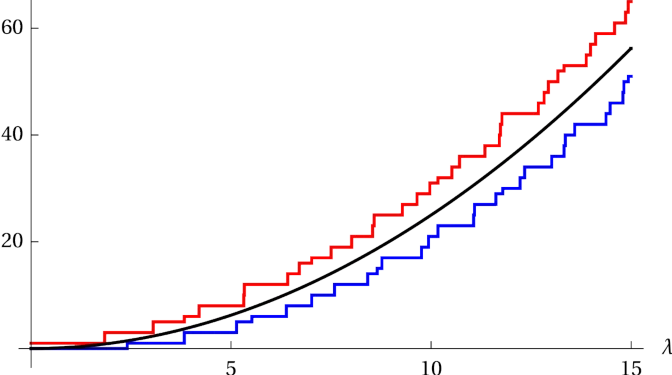
\includegraphics[width=\linewidth]{f/polyac.png}\\
		\color{darkgray}\tiny
		Filonov et al. {\bf Pólya's conjecture for Euclidean balls}, 2023
	\end{column}
	\begin{column}{0.5\linewidth}
		{\bf *} observation expérimentale des {\color{blue}"cicatrices quantiques"} associées aux trajectoires
		périodiques\\
		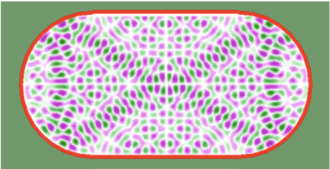
\includegraphics[width=\linewidth]{f/stascarsp.png}
	\end{column}
\end{columns}
%\begin{tabular}{ll}
%	vérification de la conjecture de Pólya~$\mathcal{N}_\Omega(\lambda)\approx\frac{\lambda^2|\Omega|}{4\pi}$ &
%	conjecture de Pólya \\
%	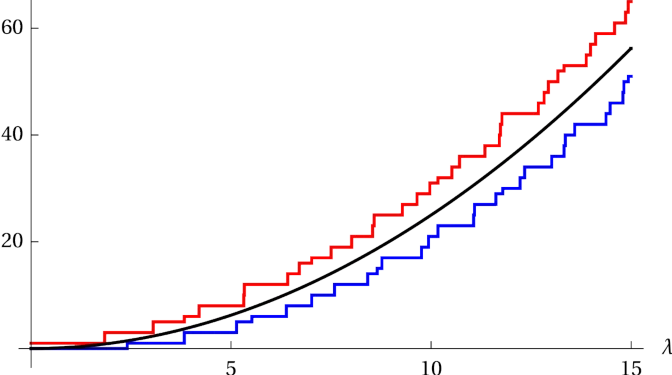
\includegraphics[width=0.37\linewidth]{f/polyac.png} &
%	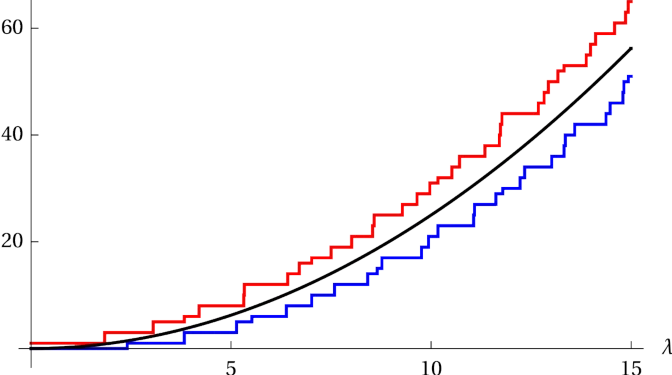
\includegraphics[width=0.37\linewidth]{f/polyac.png} \\
%\end{tabular}

\end{frame}


\end{document}


% vim:sw=2 ts=2 spell spelllang=fr:
